\chapter{Estado del arte}
\label{cap:estado}

\section{Bispectrum}

En \citet{Chael_2018} se aplicó un método de reconstrucción de imágenes utilizando el método de Máxima verosimilitud regularizada con datos \textit{closure only} (o \textit{bispectrum}. Se utiliza una antena de referencia con el objetivo de poder reducir la cantidad de posibles combinaciones y así también lograr un mejor rendimiento del software. Además se realiza una comparación con imágenes reconstruidas mediante \textit{bispectrum} y \textit{self-calibration} tanto para datos simulados como para datos de VLBA y ALMA. Sin embargo, lo realizado en \citet{Chael_2018} no está enfocado en \textit{self-calibration}. Se especifica que los pesos de los regularizadores sea óptimo y por otro lado, el método de optimización utilizado no es el mejor ya que asume diferenciabilidad. Se presentan mejores resultados que lo obtenido con el método \textit{self-calibration} junto a CLEAN, pero queda la interrogante de si \textit{self-calibration} junto a \textit{bispectrum} es una buena alternativa. Esta tesis se enfoca en este último aspecto.

Siguiendo al mismo autor, en \citet{event_horizon} se explora una variante del algoritmo MEM para observaciones obtenidas mediante \textit{Very Long Baseline Interferometry} (VLBI). Esta variante se le denomina algoritmo MEM polarimétrico, donde se combina un generador de imágenes polarizadas Stokes I que solo utiliza mediciones de bispectrum junto a generadores de imágenes Stokes Q y U que operan con relaciones polarimétricas robustas. De esto se obtienen resultados con mejor resolución que los obtenidos con CLEAN, cuando se trata de imágenes de distribuciones de fuentes suaves y compactas. 

En \citet{m87} se estudia la variabilidad de las imágenes reconstruidas para el agujero negro ubicado en el centro de la galaxia M87. Para esto se utilizan datos del tipo \textit{closure phases} o \textit{bispectrum}, de tal manera de analizar la variabilidad que tienen estos datos. De esto se obtuvo que los únicos triángulos que presentaban una gran variabilidad ($\sim$90 - 180$^o$) son aquellos cuyas baselines cruzan la amplitud de visibilidad mínima en el plano $uv$. Aún así se encuentra que tres triángulos presentan poca variabilidad ($\sim$3 - 5$^o$). 

\textit{Bispectrum} también a sido estudiado en \citet{geometry}. En este se muestra el principio de conservación forma-orientación-tamaño o SOS por su traducción al ingles, donde se dice que, la cualidad de que las \textit{closure-phases} no esten afectadas por el ruido multiplicativo esta relacionada a la forma y orientación del triangulo entre las tres antenas. El principio de conservación SOS permite la aplicación de dos métodos para obtener los datos \textit{closure phases} directamente desde el plano de la imagen. El primero permite estimarlo geométricamente en el plano de la imagen a partir de una única medición de cualquiera de las alturas del triangulo delimitado por las tres franjas principales. El segundo permite la estimación a partir de una relación invariante que existe entre la \textit{closure phase} al cuadrado y el productor de las áreas encerradas por la triada de elementos en el plano de apertura y el triangulo encerrado por las tres franjas en el plano de la imagen. 

Una nueva técnica para síntesis de imágenes es propuesta en \citet{akiyama2017imaging} donde se propone utilizar la amplitud de las visibilidades y el \textit{closure phase} a través de las funciones de regularización $\ell_{1}$-norm y la variación total (TV) de la distribución del brillo, así como también la técnica \textit{cross-validation} (CV) para obtener los mejores valores para los parámetros $\eta_{l}$ y $\eta_{t}$. Para la realización de esto se minimiza la ecuación \ref{eq:paper_min}. 

\begin{equation}
    \label{eq:paper_min}
    C(I) = \chi^{2}(I) + \eta_{l} ||I||_{1} + \eta_{t} ||I||_{tv}
\end{equation}

El primer término de esta representa la desviación entre la imagen reconstruida y las visibilidades observadas. Este término esta dado por la ecuación \ref{eq:aki_eq1} donde $A(FI)$ y $B(FI)$ representan los operadores para calcular las amplitudes y las \textit{closure phases}. El segundo término representa la regularización tipo LASSO usando $\ell_{1}$-norm y el tercer término representa la regularización TV definida por la ecuación \ref{eq:aki_eq2}.

\begin{equation}
    \label{eq:aki_eq1}
    \chi^{2}(I) = || \bar{V} - A(FI)||^{2}_{2} + || \Psi - B(FI) ||^{2}_{2}
\end{equation}

\begin{equation}
    \label{eq:aki_eq2}
    ||I||_{tv} = \sum_{i} \sum_{j} \sqrt{|I_{i+1j} - I_{ij}|^{2} + |I_{ij+1} - I_{ij}|^{2}}
\end{equation}

Finalmente, los resultados obtenidos indican que se puede alcanzar una resolución óptima de $\sim20\% - \sim30\%$ del límite de difracción $\lambda / D_{max}$ que es la resolución espacial nominal del radio-interferometro. Sin embargo, una acotación hecha es que este método se podría mejorar utilizando \textit{self-calibration} debido a la perdida de información que se sufre a utilizar técnicas como \textit{closure-phases}. 

\textit{Bispectrum} es utilizado en \citet{bowersobservations} para reconstruir imágenes de sistemas de estrellas binarias, esto para así aprovechar eliminar el ruido atmosférico que puedan tener las imágenes. El objetivo de este articulo es determinar si las estrellas observadas son estrellas dobles físicas o par binario, que son aquellas estrellas conformadas por una mas brillante que la otra y orbitan alrededor de un baricentro. Para esto se utilizaron los datos de \textit{Boyce Astro Robotic Observatory} que consisten entre 500 a 1000 imágenes con una exposición entre 0.01 a 1 segundos. Las imágenes obtenidas se pueden observar en la Figura \ref{fig:bin_star}. Los resultados indican que las observaciones 3 y 7 están atados gravitacionalmente mientras que 1 y 2 no lo están, por otro lado, las observaciones 4, 6 y 8 son binarios pero con la observación 5 se mantiene en duda debido a que el resultado obtenido difiere significativamente con los datos históricos de esta observación. 

\begin{figure}[!ht]
	\centering
	\captionsetup{justification=centering}
	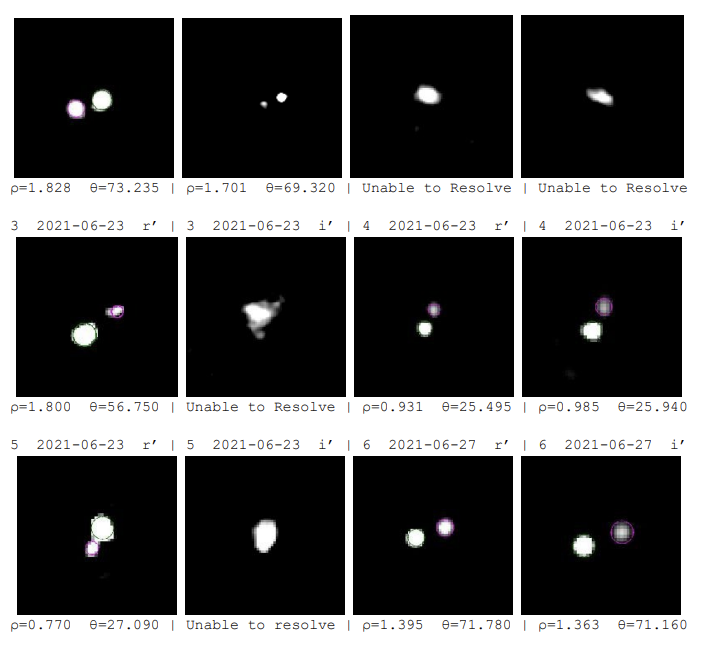
\includegraphics[scale=0.6]{images/pares_estrellas.png}
	\caption[Sistema de estrellas binarias]{Imágenes obtenidas mediante el método de Bispectrum para sistema de estrellas binarias. Cada subfigura contiene la estrella más brillante (círculo verde) y la menos brillante (círculo morado), así como también la separación ($\rho$) y ángulo ($\theta$) para cada observación. Fuente: \citep{bowersobservations}}
	\label{fig:bin_star}
\end{figure}

\section{Self-calibration}

El método de \textit{self-calibration} es utilizado en \citet{cook_seymour_sokolowski_2021} para la calibración de datos obtenidos por el proyecto \textit{Murchinson Widefield Array} (MWA). En altas frecuencias aparecen \textit{sidelobes}, que dificultan el procesamiento de la imagen y la calibración, donde para MWA esto ocurre a los $\sim$ 350 MHz. Sin embargo, en este trabajo se propone un nuevo método de calibración donde se crea un modelo del cielo que ha sido interpolado en altas y bajas frecuencias, el cual es sometido a un ciclo de \textit{self-calibration} que es utilizado para crear una mascara de las visibilidades. Esto abre las posibilidades de poder trabajar a frecuencias de 300 MHz para MWA. 

En \citet{ortiz} se estudia la forma intrínseca del agujero negro supermasivo Sagitario A*, que se encuentra en el centro de la Vía Láctea. En este se realiza una comparación entre lo obtenido con solamente \textit{closure amplitudes} y lo obtenido con \textit{self-calibration}. De los análisis realizados se da a conocer que ambos enfoques son adecuados para obtener resultados consistentes 

\begin{comment}
    Una implementación en GPU puede ser encontrada en \citet{GPU}, donde realiza una implementación de un algoritmo \textit{bispectrum} con usos de GPU. En este se realiza una comparación para la obtención de \textit{radio transients}, que son estallidos de radiación electromagnética, de una implementación multi-thread en CPU y una implementación GPU con CUDA. Esto da como resultado que el algoritmo \textit{bispectrum} es eficiente tanto en CPU como GPU, donde el primero obtuvo un \textit{speed-up} de 3.2x y el segundo obtuvo un \textit{speed-up} 20 veces mas que el primero. 
\end{comment}

\textit{Common Astronomy Software Applications} (CASA) \citep{bean2022casa} es el principal software utilizado para los observatorios ALMA y VLA, aunque también utilizado en otros observatorios. Este software es capaz de manejar datos telescópicos, donde su principal objetivo es la calibración de estos y la reconstrucción de imágenes con estos. De esta manera, en CASA se puede encontrar una implementación para el método de \textit{self-calibration}, sin embargo no es posible encontrar una implementación para el método de \textit{Bispectrum}. Aunque el primer método es mayormente utilizado mediante este software, este tiene que ser ejecutado por el experto de manera manual, es decir, ejecutar comando por comando todo el algoritmo presentado en la sección \Ref{sec:selfcal}. Un script de ejemplo para esto puede ser encontrado en el Anexo \ref{finales:anexo2}, así como también una imagen resultante de todo el proceso se puede ver en la Figura \ref{fig:selcal_comp}.

\begin{figure}
 \centering
  \subfloat[Imagen residual original]{
   \label{fig:original}
    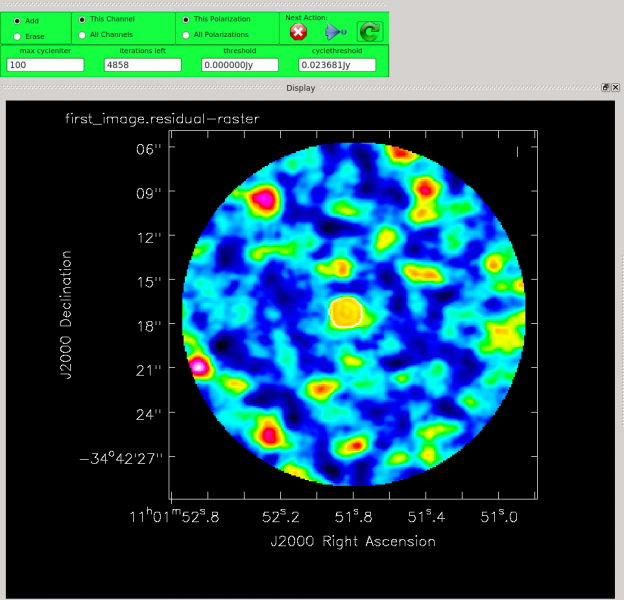
\includegraphics[width=0.4\textwidth]{images/original_casa.png}}
  \subfloat[Imagen residual luego de cuatro ciclos]{
   \label{fig:four}
    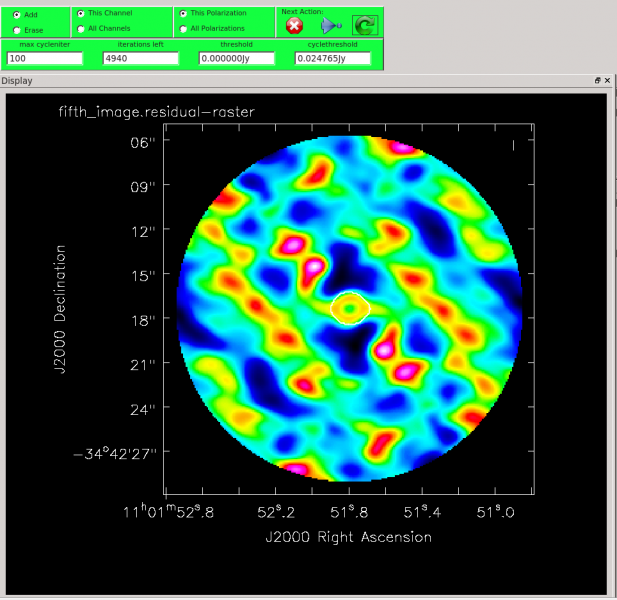
\includegraphics[width=0.4\textwidth]{images/four_self_casa.png}}
 \caption[Imagenes residuales CASA self-calibration]{Imágenes residuales de conjunto de datos TWHydra. Fuente: \citep{CASA_self_cal}.}
 \label{fig:selcal_comp}
\end{figure}

En \cite{FernandezTesis} se presenta una implementación de \textit{self-calibration} utilizando redes neuronales profundas a través de \textit{Amazon Web Services (AWS)}. Se entrena una red con imágenes perturbadas con un error conocido, donde se es capaz de predecir el error que tenga el conjunto de datos. Las redes entrenadas son iguales a las cantidades de antenas y se selecciona la predicción que presente la mayor mejora en la imagen mediante la comparación del valor del PSNR. De esto se obtiene un método automatizado y factible que es capaz de obtener mejoras en imágenes utilizando \textit{self-calibration}. Un resultado obtenido se puede observar en la Figura \ref{fig:tesis_fer}.

\begin{figure}[!ht]
	\centering
	\captionsetup{justification=centering}
	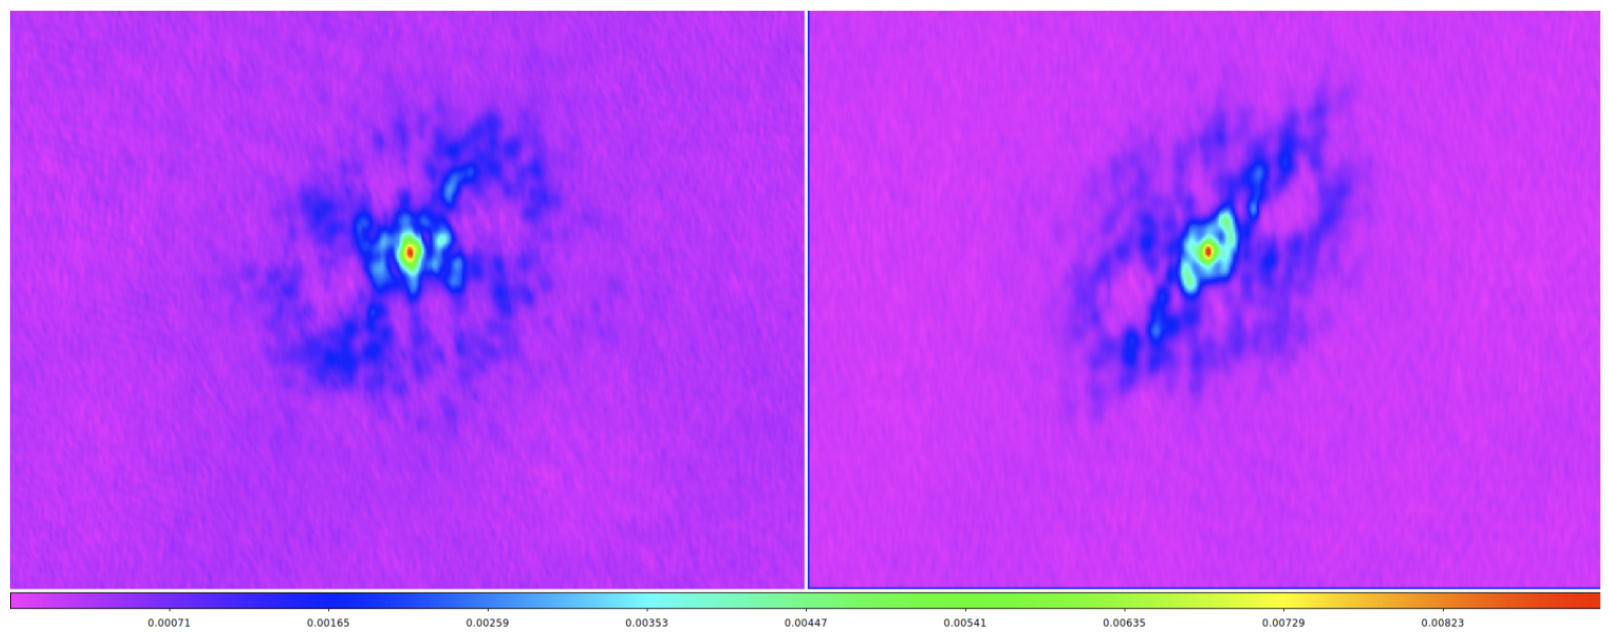
\includegraphics[scale=0.3]{images/self_cal_tesis.png}
	\caption[Resultado de Selfcal con redes neuronales]{HL-TAURI con ruido (izquierda) y con Selfcal (derecha). Fuente: \citep{FernandezTesis}}
	\label{fig:tesis_fer}
\end{figure}
